\documentclass[11pt,a4paper]{article}

\usepackage{ctex}
\usepackage{graphicx} % Required for the inclusion of images
\usepackage{subfigure} % Required for the inclusion of images
\usepackage{natbib} % Required to change bibliography style to APA
\usepackage{amsmath} % Required for some math elements 
\usepackage{listings}
\usepackage{xcolor}
\usepackage{indentfirst}
\usepackage{geometry}

\geometry{a4paper,scale=0.8}

\title{\textbf{Project0: Compiling Linux Kernel}} % Title
\author{518021911193,刘昊林} % Author name and email
\date{} % Date for the report

\begin{document}
	\maketitle % Insert the title, author and date
	
	\section{准备阶段}
	下载VMware Workstation Pro软件,下载Ubuntu操作系统镜像文件ubuntu-16.04.6-desktop-amd64.iso。然后在VMware中安装一个新的虚拟机。\par
	打开虚拟机,在终端中输入uname -a命令,可以看到当前Ubuntu系统中自带的Linux内核版本为Linux Ubuntu 4.15.0-88-generic。具体内容如下图所示:
	\begin{figure}[h]
		\centering
		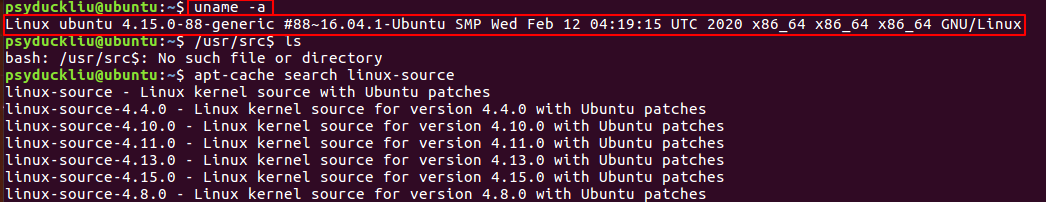
\includegraphics[width=0.7\linewidth]{Pictures/1_WPS}
		\caption{查看当前内核信息}
		\label{fig:1wps}
	\end{figure} \par
	然后登陆www.kernel.org下载Linux内核源码,我这里下载的是4.19.108版内核,下载完成后对压缩包进行解压。这里我使用的是sudo tar -xavf linux-4.19.108.tar.xz -C /usr/src命令,将解压好的文件直接送入/usr/src文件夹下。并且在解压完成后还可以使用cd /usr/src命令进入该文件夹,然后使用ls命令就可以看到已经解压后的linux-4.19.108文件。具体内容如下图所示:
	\begin{figure}[h]
		\centering
		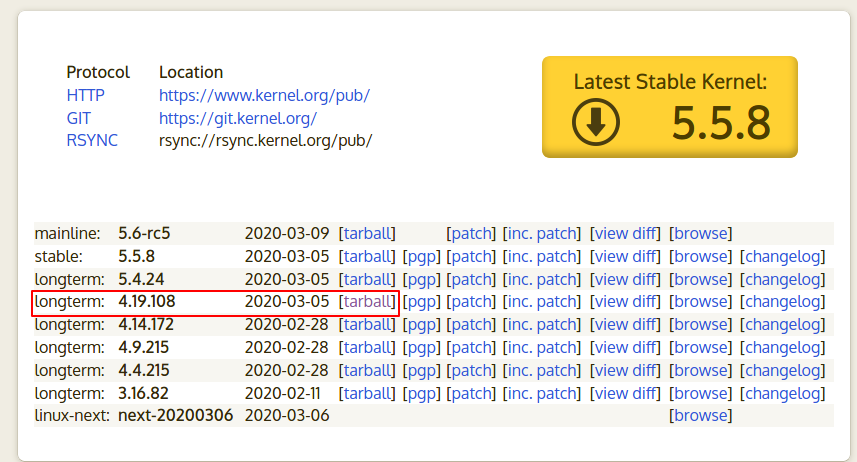
\includegraphics[width=0.7\linewidth]{Pictures/3_WPS}
		\caption{选择下载的Linux内核版本}
		\label{fig:3wps}
	\end{figure}
	\newpage
	\begin{figure}[h]
		\centering
		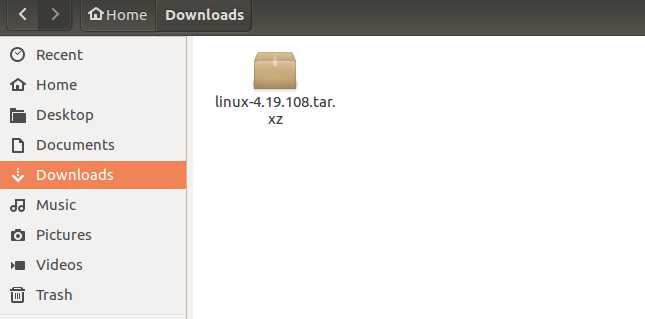
\includegraphics[width=0.7\linewidth]{Pictures/2}
		\caption{下载好的Linux源码压缩包}
		\label{fig:2}
	\end{figure}
	\begin{figure}[h]
		\centering
		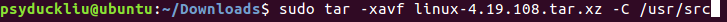
\includegraphics[width=0.7\linewidth]{Pictures/4}
		\caption{解压源码压缩包}
		\label{fig:4}
	\end{figure}
	\begin{figure}[h]
		\centering
		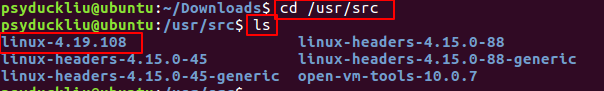
\includegraphics[width=0.7\linewidth]{Pictures/5_WPS}
		\caption{进入/usr/src文件夹检查解压结果}
		\label{fig:5wps}
	\end{figure}

	\section{安装编译内核需要的一些程序}
	首先输入sudo apt-get upgrade命令,更新软件来源,否则可能会出现安装失败的情况。\par
	再依次输入以下命令,来下载必要程序:\par
	sudo apt-get install libncurses5-dev openssl libssl-dev\par 
	sudo apt-get install build-essential openssl\par 
	sudo apt-get install pkg-config\par 
	sudo apt-get install libc6-dev\par 
	sudo apt-get install bison\par 
	sudo apt-get install flex\par 
	sudo apt-get install libelf-dev\par 
	sudo apt-get install zlibc minizip\par 
	sudo apt-get install libidn11-dev libidn11\par 
	具体内容如下图所示(只选择了一部分程序的下载截图):
	\newpage
	\begin{figure}[h]
		\centering
		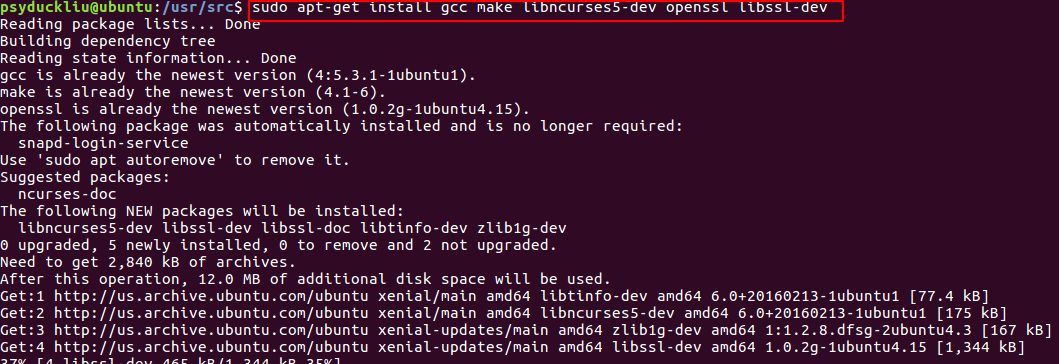
\includegraphics[width=0.7\linewidth]{Pictures/6_WPS}
		\caption{下载必要程序(1)}
		\label{fig:6wps}
	\end{figure}
	\begin{figure}[h]
		\centering
		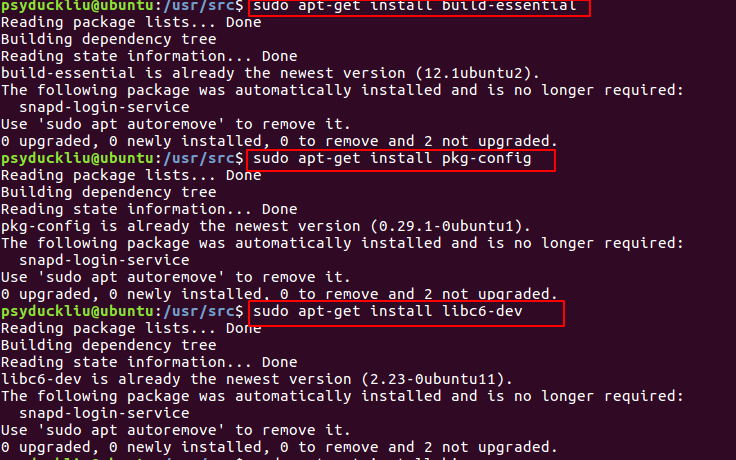
\includegraphics[width=0.7\linewidth]{Pictures/8_WPS}
		\caption{下载必要程序(2)}
		\label{fig:8wps}
	\end{figure}

	\section{编译内核前的一些准备}
	在终端中依次输入以下三条命令:\par
	sudo make mrproper\par 
	sudo make clean \par
	sudo make menuconfig\par
	在这其中,sudo make mrproper是为了清除编译过程中产生的所有中间文件;sudo make clean是为了清除上一次产生的编译中间文件;sudo make menuconfig是为了对内核选项进行配置,在这里我直接选择了exit退出,保留默认设置。\par
	具体内容如下图所示:
	\newpage
	\begin{figure}[h]
		\centering
		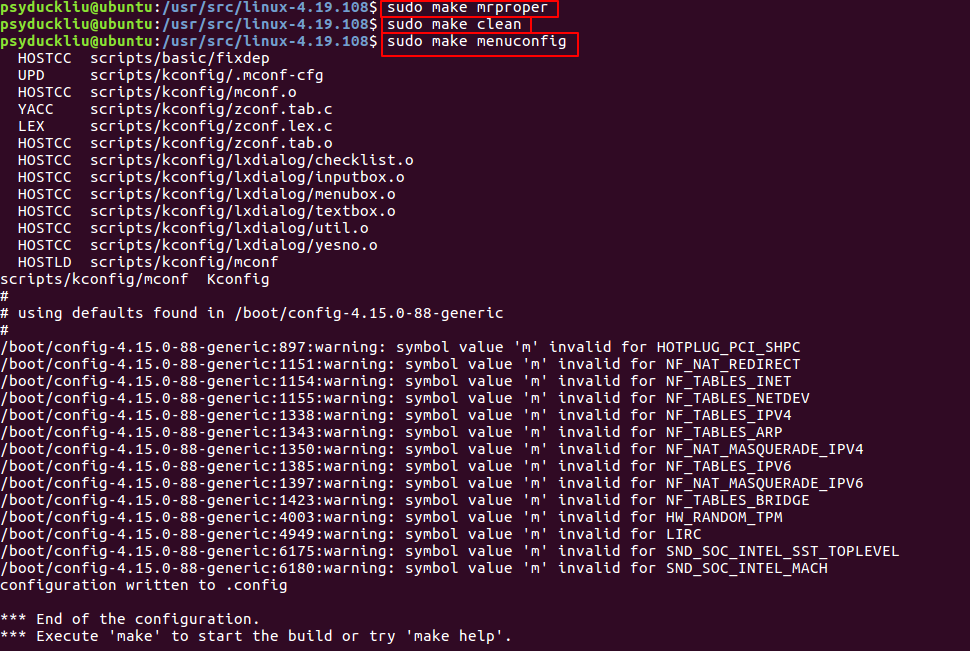
\includegraphics[width=0.7\linewidth]{Pictures/15_WPS}
		\caption{依次输入三条命令}
		\label{fig:15wps}
	\end{figure}
	\begin{figure}[h]
		\centering
		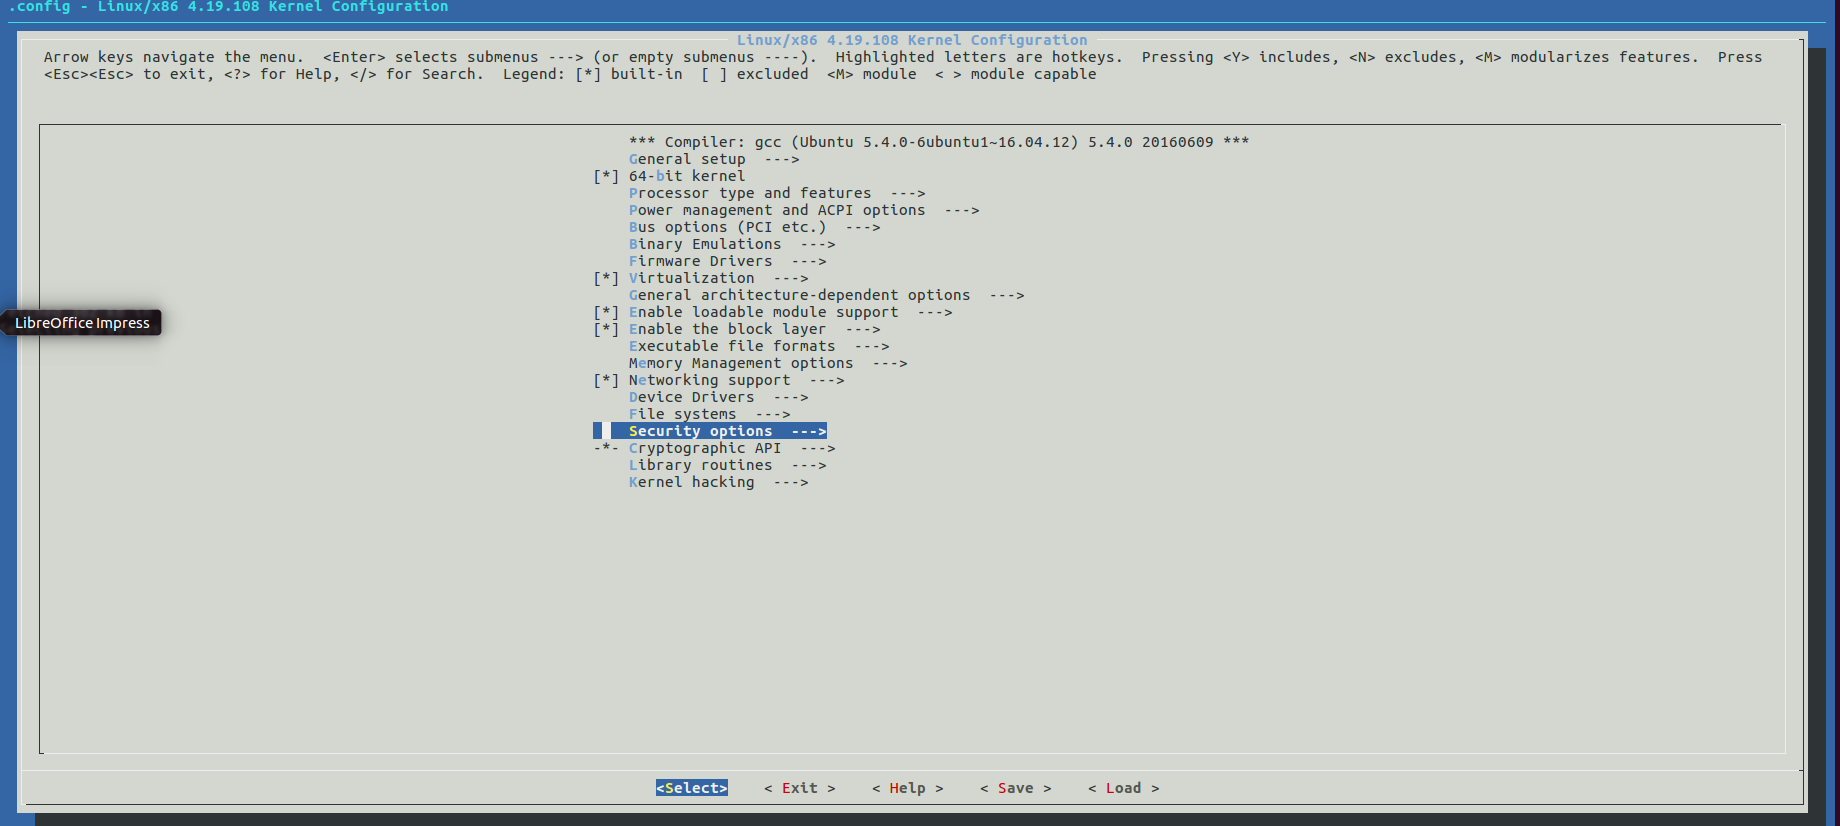
\includegraphics[width=0.7\linewidth]{Pictures/14}
		\caption{sudo make menuconfig的配置界面}
		\label{fig:14}
	\end{figure}
	
	\section{编译内核}
	在终端中输入命令:sudo make –j2,我在这里采用了2个线程并行编译的方法,来加快编译速度,但是编译内核的过程还是花费了3个小时。并且在编译过程中还出现了gcc: internal compiler error: Killed (program cc1plus)”这样的错误。经过在CSDN上的搜索了解,我知道这个错误出现的原因是内存不足,所以我把虚拟机关机,把内存从原来的2GB调整到了4GB,再打开虚拟机,就可以顺利地继续进行编译了。\par
	具体内容如下图所示:
	\newpage
	\begin{figure}[h]
		\centering
		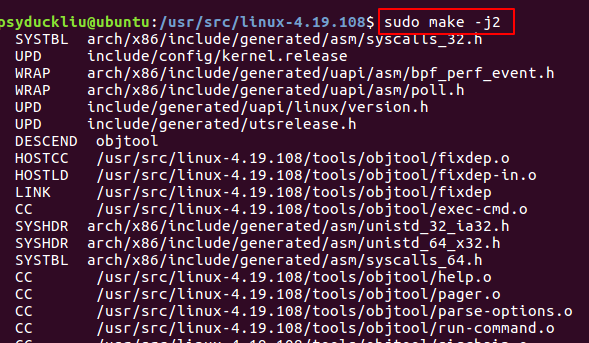
\includegraphics[width=0.7\linewidth]{Pictures/17_WPS}
		\caption{sudo make –j2,开始编译}
		\label{fig:17wps}
	\end{figure}
	\begin{figure}[h]
		\centering
		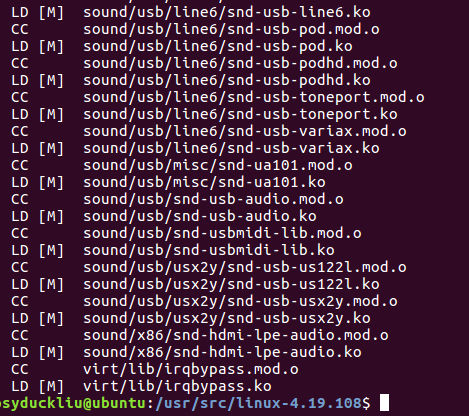
\includegraphics[width=0.5\linewidth]{Pictures/18}
		\caption{编译结束}
		\label{fig:18}
	\end{figure}

	\section{安装内核模块和内核}
	在终端中依次输入以下两条命令:\par
	sudo make modules\_install\par       
	sudo make install\par
	其中sudo make modules\_install安用于安装内核模块;sudo make install用于安装内核。都安装好之后,再输入reboot命令,重启虚拟机,就安装完成了。具体内容如下图所示:
	\newpage
	\begin{figure}[h]
		\centering
		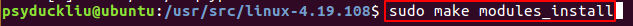
\includegraphics[width=0.7\linewidth]{Pictures/19_WPS}
		\caption{sudo make modules\_install,开始安装内核模块}
		\label{fig:19wps}
	\end{figure}
	\begin{figure}[h]
		\centering
		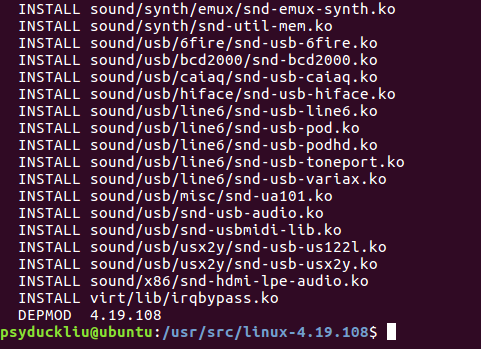
\includegraphics[width=0.7\linewidth]{Pictures/20}
		\caption{安装内核模块结束}
		\label{fig:20}
	\end{figure}
	\begin{figure}[h]
		\centering
		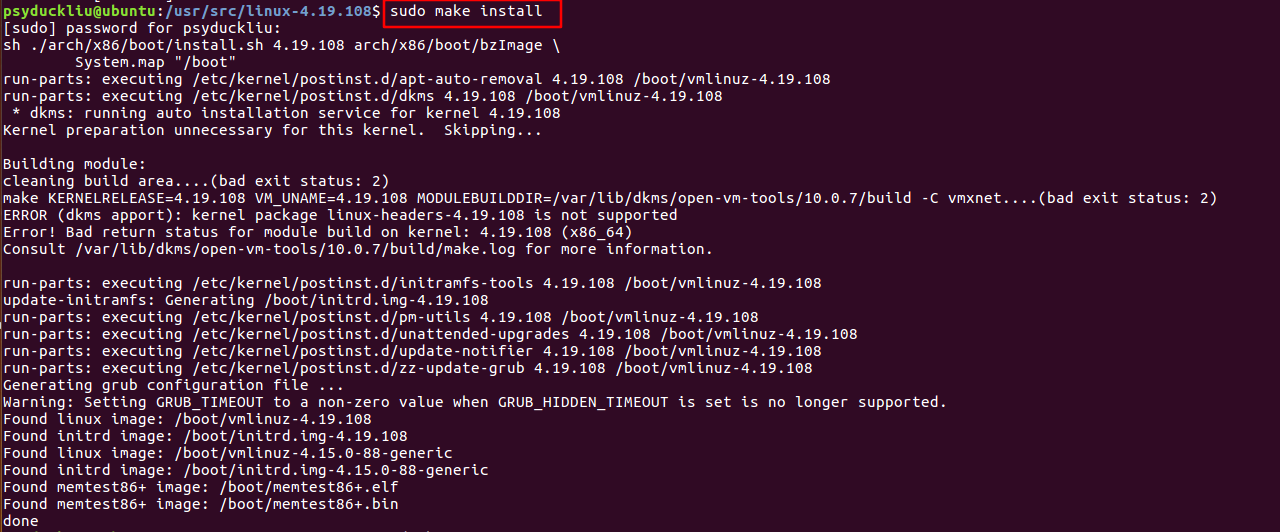
\includegraphics[width=0.5\linewidth]{Pictures/22_WPS}
		\caption{sudo make install,安装内核}
		\label{fig:22wps}
	\end{figure}

	\section{检查新内核,卸载旧内核}
	在终端输入uname -a命令,就可以发现内核已经是新编译的Linux Ubuntu 4.19.108了。再输入sudo dpkg --get-selections | grep 'linux'命令,就可以查找到所有的内核信息,我们可以再输入sudo apt-get purge linux-image-4.15.0.88命令删除不再需要的内核。\par
	具体内容如下图所示:
	\newpage
	\begin{figure}[h]
		\centering
		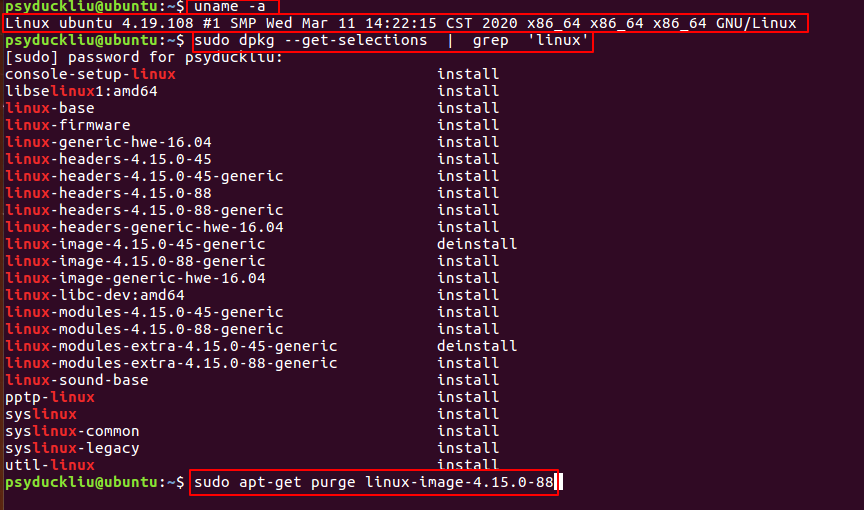
\includegraphics[width=0.7\linewidth]{Pictures/24_WPS}
		\caption{检查新内核,卸载旧内核}
		\label{fig:24wps}
	\end{figure}
	
	
	
	
	
	
	
	
		
	
	
	
	
	
	
	
	

\end{document}